\documentclass{article}\usepackage{amsmath,amssymb,amsthm,tikz,tkz-graph,color,chngpage,soul,hyperref,csquotes,graphicx,floatrow}\newcommand*{\QEDB}{\hfill\ensuremath{\square}}\newtheorem*{prop}{Proposition}\renewcommand{\theenumi}{\alph{enumi}}\usepackage[shortlabels]{enumitem}\usepackage[nobreak=true]{mdframed}\usetikzlibrary{matrix,calc}\MakeOuterQuote{"}\usepackage[margin=0.75in]{geometry} \newtheorem{theorem}{Theorem}

\title{CS70 - Lecture 10 Notes}
\author{Name: Felix Su$\quad$SID: 25794773}
\date{Spring 2016$\quad$GSI: Gerald Zhang}
\begin{document}
\maketitle

%%%% Topic %%%%
\subsection*{Polynomials}
%%%% Notes %%%%
\begin{itemize}
\item \textbf{Fact}: Any $d+1$ points specifies a distinct degree $d$ polynomial 
\item \textbf{Modular Fact}: Any $d+1$ points specifies a distinct degree $d$ polynomial in mod $p$ space when $p$ is prime
\item \textbf{Uniqueness Fact}: At most one degree $d$ polynomial hits $d+1$ points\\
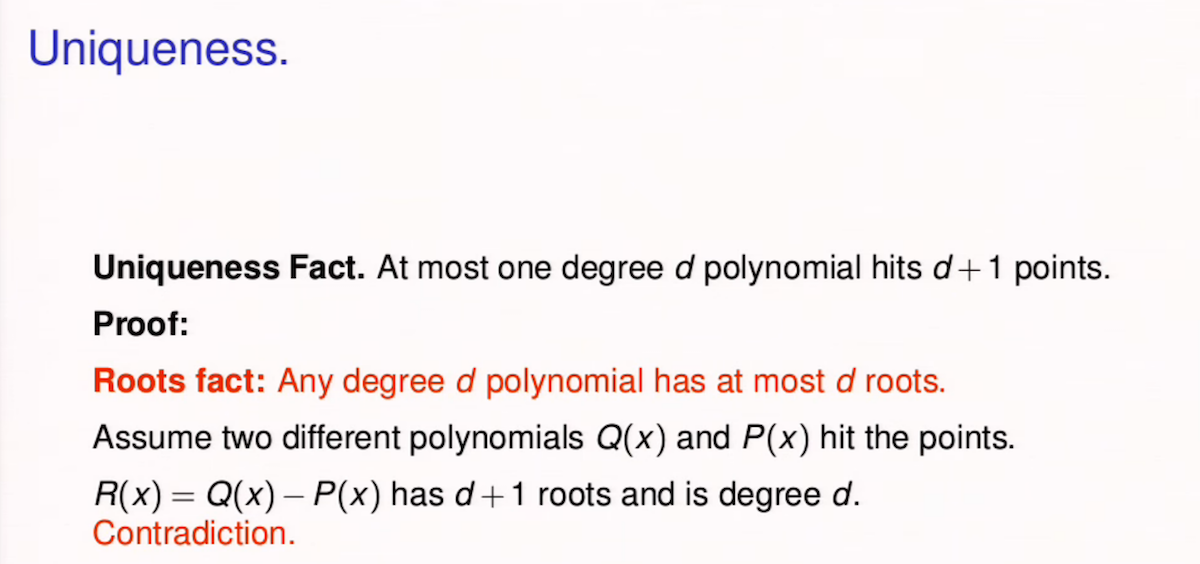
\includegraphics{uniquefact}
\item \textbf{Roots Fact}: Any degree $d$ polynomial has at most $d$ roots\\
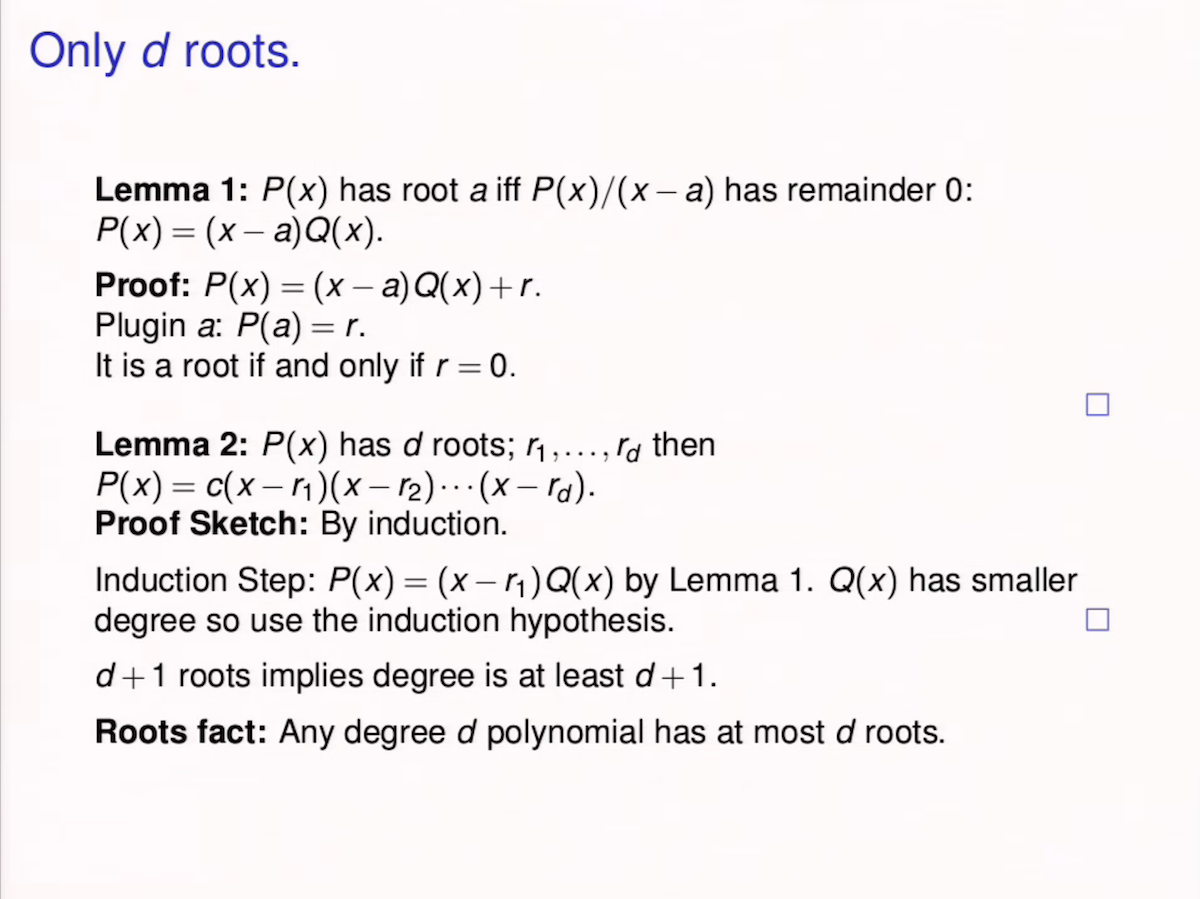
\includegraphics{rootsfact}
\end{itemize}
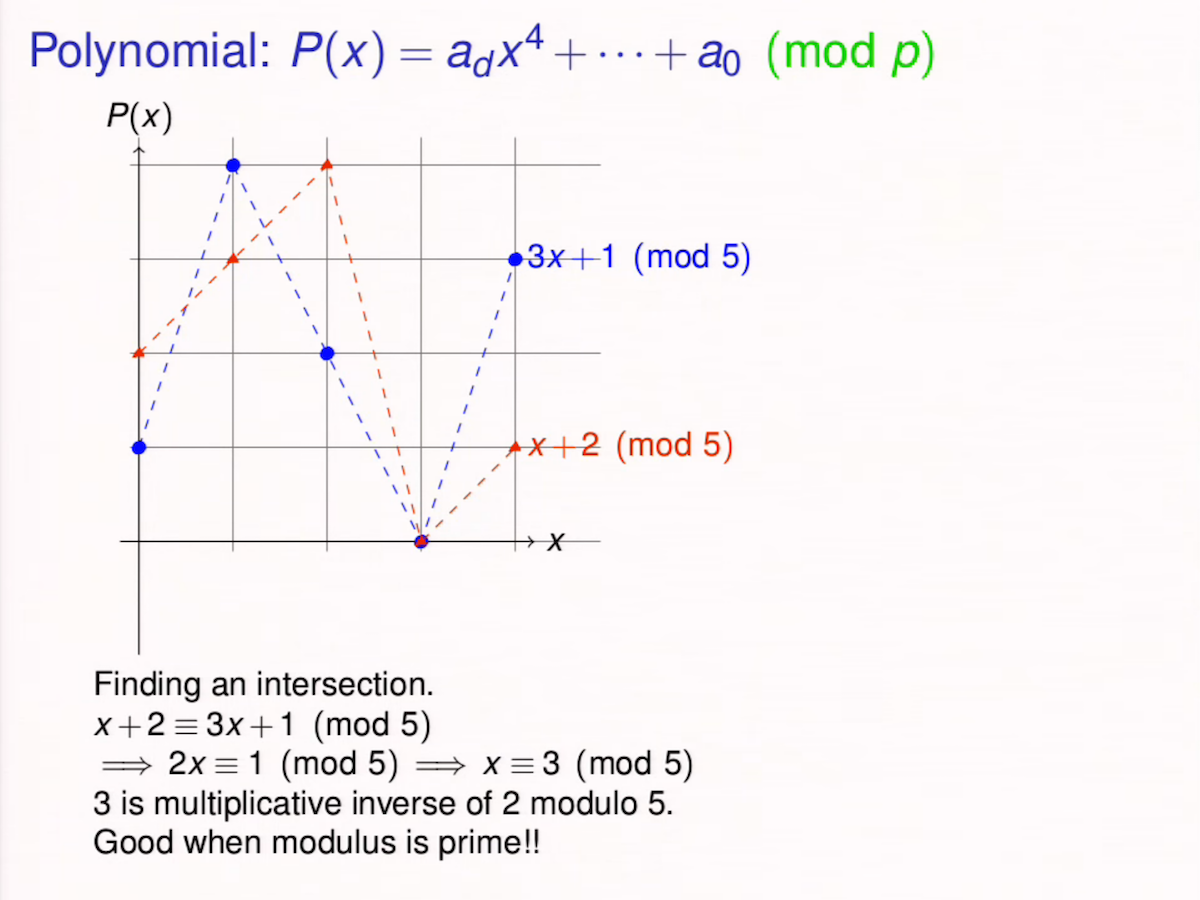
\includegraphics{modpoly}\\
\begin{itemize}
\item Polynomials only map to f(x) at integer values of x
\item f(x) is contained in the mod space
\item Use delta functions to create meaningful polynomials in mod space
\end{itemize}
\textbf{Shamir's $k$ out of $n$ scheme:}\\
Secret $s \in \{0, ..., p-1\}$\\
Set $a_0 = s$, randomly assign $a_1, ..., a_{k-1}$\\
Let $P(x) = a_{k-1}x^{k-1} + a_{k-2}x^{k-2} + ... + a0$ with $P(0) = a_0 = s$\\
Share $(i, P(i) \bmod p)$ with $i$-th person\\
$k$ shares gives secret (degree $= d = k-1$, Modular fact, $d+1 = k$ shares gives the polynomial which reveals $P(0) = s$\\
\textbf{Solve for polynomial given $d+1$ coordinates}\\
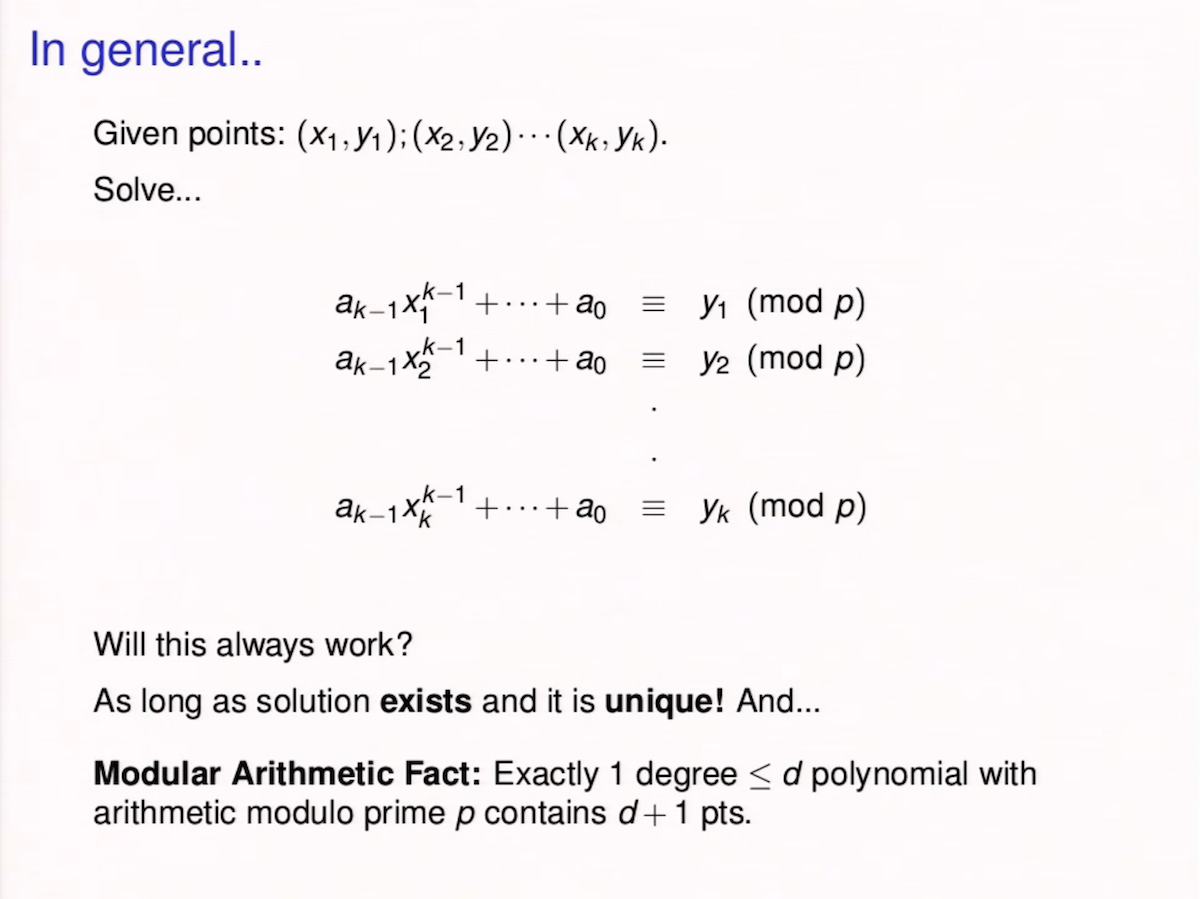
\includegraphics{genpoly}
\begin{itemize}
\item $d = k-1, d+1 = k$
\item Solve system of linear equations to get $a_0$
\end{itemize}

%%%% Topic %%%%
\subsection*{Lagrange Interpolation}
%%%% Notes %%%%
\textbf{Delta Function}
$$
\Delta_i(x) =
\begin{cases}
1, & x =x_i \\
0, & x =x_j \text{ for } j\ne i \\
\text{doesn't matter}, & x = \text{anything else}
\end{cases}
$$
\begin{itemize}
\item 1 at one point (x-value), 0 everywhere else
\item valid for a set of x values $x_1, ..., x_{d+1}$
\item $y_i\Delta_i(x) = y_i$ because $\Delta_i(x)$ is 1 at $x_i$ and 0 everywhere else
	\begin{itemize}[label=$\star$]
	\item $P(x) = y_1\Delta_1(x) + y_2\Delta_2(x) + ... + y_{d+1}\Delta_{d+1}(x)$ because at $x_i$ you only get $y_i$ ($\Delta{x_i}$ is 0 at anything except $x_i$)
	\end{itemize}
\begin{mdframed}
\textbf{Formation of Delta Function}:\\
Given points: $(x_1, y_1); (x_2, y_2); ... (x_{d+1}, y_{d+1})$\\\\
\begin{equation}\Delta_i(x) = \frac{\prod_{j\ne i}(x-x_j)}{\prod_{j\ne i}(x_i-x_j)}\end{equation}
\end{mdframed}
\end{itemize}